\section*{METODOLOGIA}

O pipeline analítico inicia-se pelo saneamento contínuo dos dados brutos do INPE, aplicando validações de esquema, descarte de leituras duplicadas e eliminação de inconsistências na telemetria satelital. Para reduzir o tempo de processamento espacial em comparação a bancos relacionais convencionais, o cálculo de distâncias relativas às malhas territoriais (rodovias do DNIT, hospitais do CNES, terras da FUNAI e municípios do IBGE) é antecipado diretamente em memória durante a etapa de ingestão.

Para estruturar os dados pontuais, empregam-se algoritmos espaciais específicos: o \textbf{\textit{DBSCAN}} agrupa focos contíguos no espaço e no tempo para delimitar perímetros de queima, enquanto grafos no \textbf{\textit{NetworkX}} representam a malha elétrica do SIN (ONS), estimando o risco de desligamentos e falhas em cascata em linhas e subestações.

\begin{center}
    \vspace{-0.10cm}
    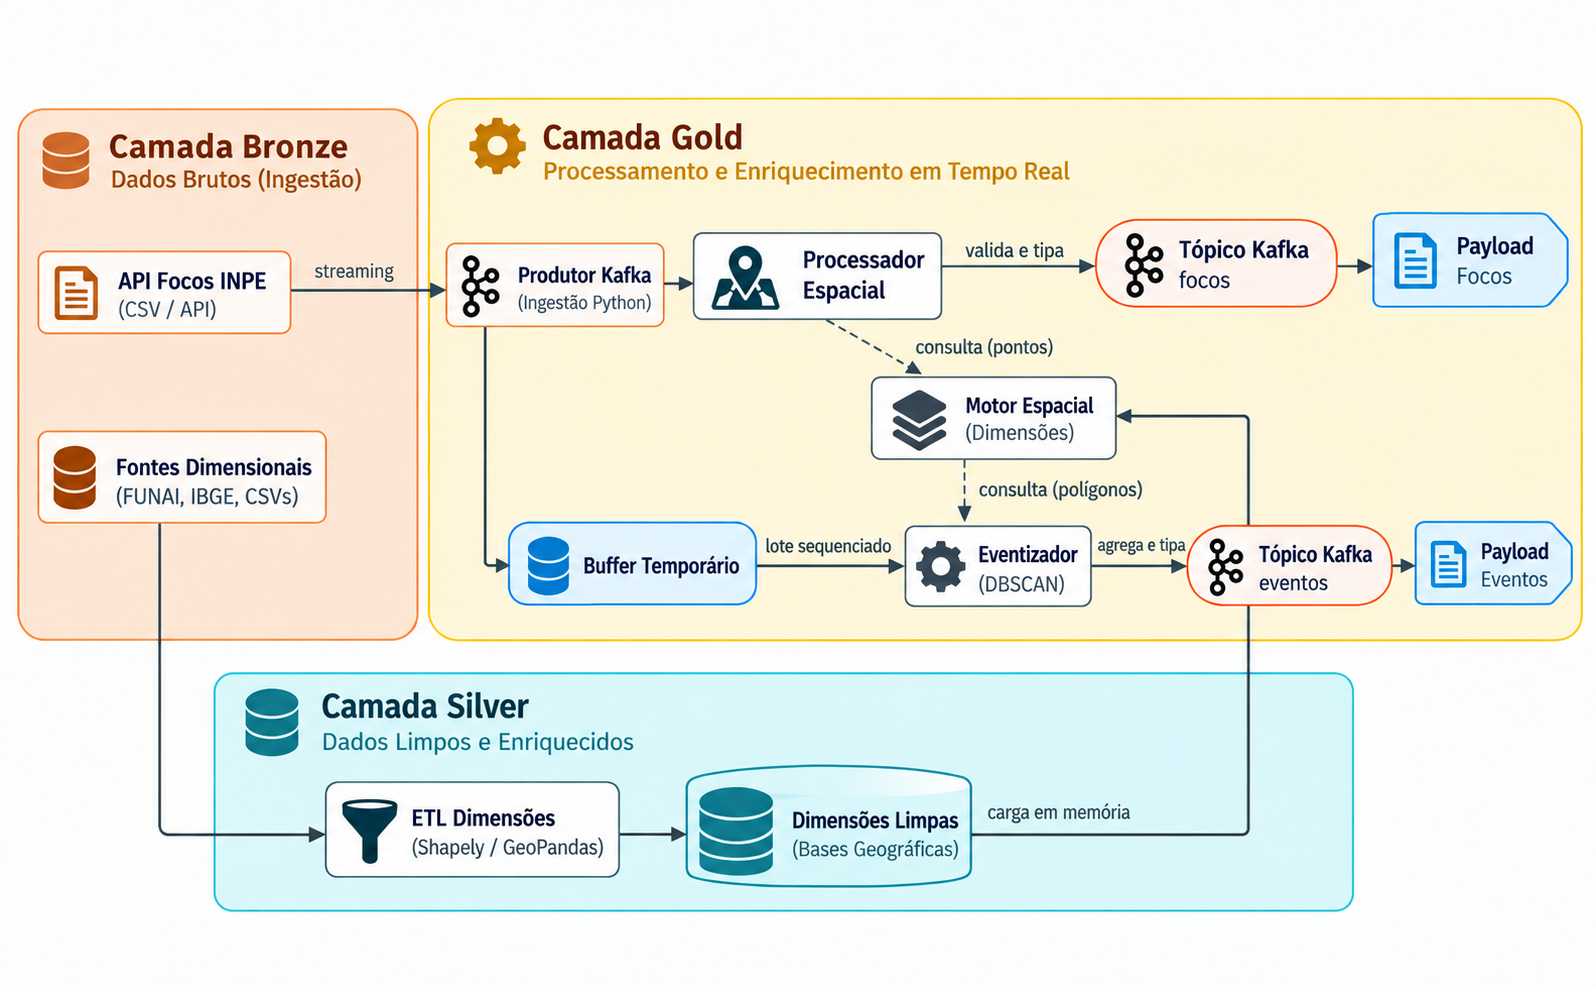
\includegraphics[width=0.55\linewidth]{fig_pipeline_camadas.png}
    \captionof{figure}{Pipeline de ingestão e processamento espacial em memória.}
    \vspace{-0.10cm}
\end{center}

Os eventos enriquecidos alimentam o \textbf{\textit{Apache Kafka}}, que organiza o fluxo de dados entre o registro individual de focos e o encaminhamento de polígonos agregados para a camada analítica.

Na etapa de armazenamento, as mensagens são consumidas pelo banco colunar distribuído \textbf{\textit{Apache Druid}} (YANG et al., 2014). O modelo dimensional adota identificadores numéricos e tabelas de consulta rápida em memória, viabilizando agregações geográficas com menor tempo de resposta (Fig. 2).

\begin{center}
    \vspace{-0.10cm}
    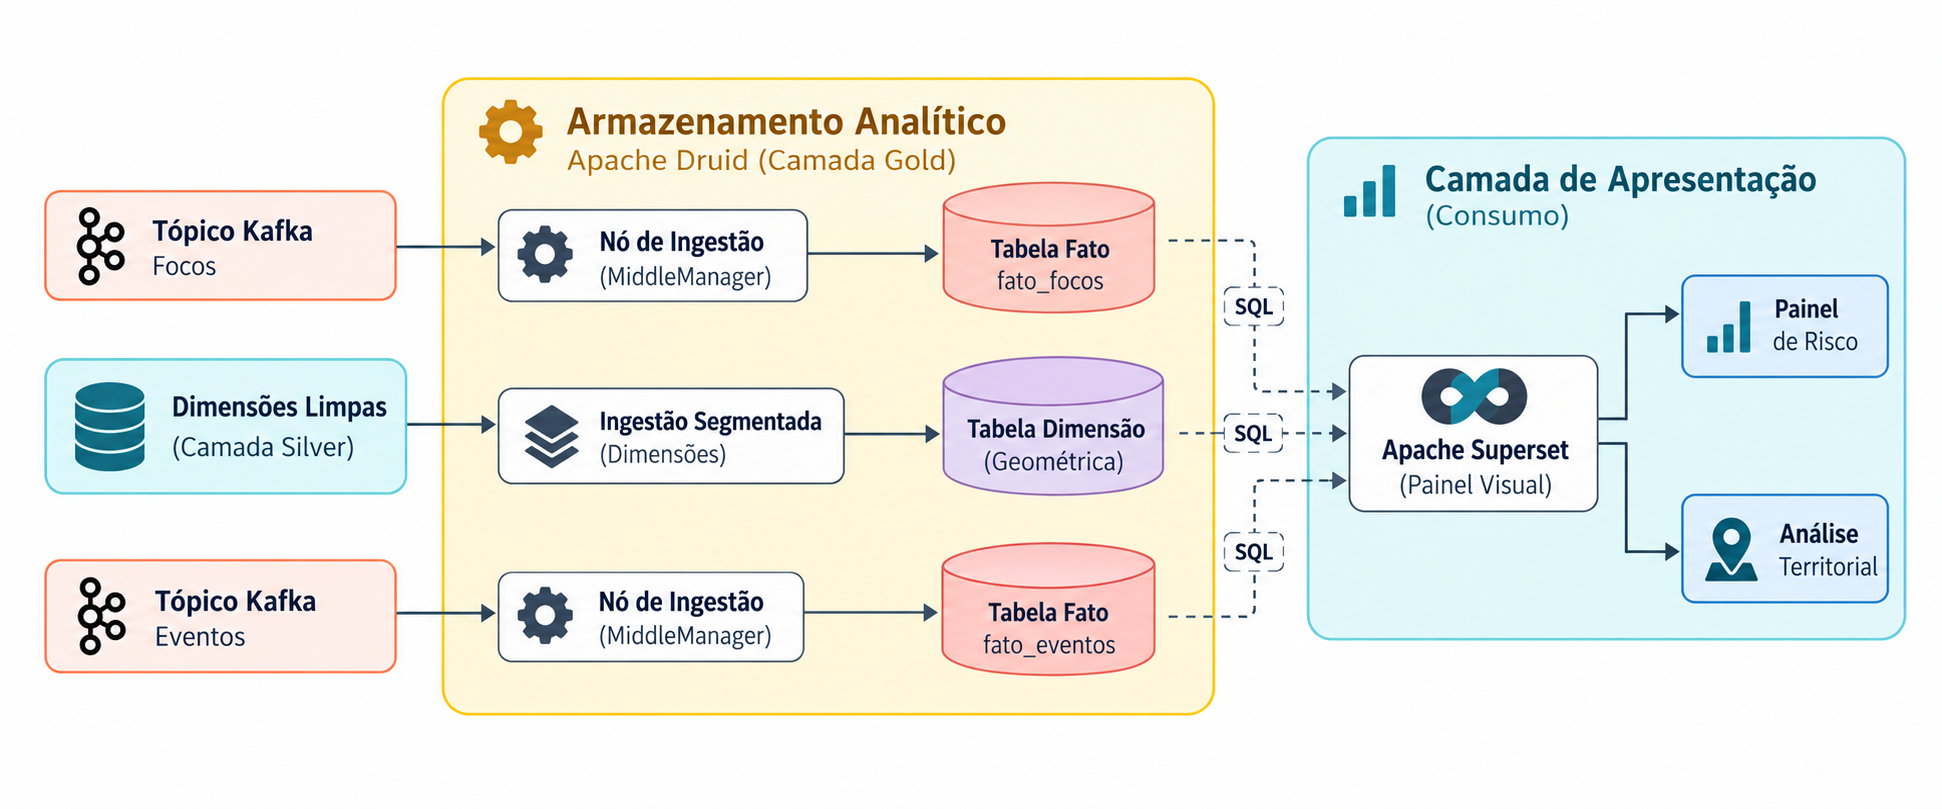
\includegraphics[width=0.55\linewidth]{fig_druid_superset.png}
    \captionof{figure}{Arquitetura analítica com Apache Druid e Apache Superset.}
    \vspace{-0.10cm}
\end{center}

A camada de visualização no \textbf{\textit{Apache Superset}} organiza as métricas em painéis temáticos (visão geral, saúde, terras indígenas e energia), estruturando os dados para suporte à tomada de decisão operacional.
